\documentclass[aspectratio=169]{beamer}
\usetheme{Madrid}
\usecolortheme{default}

\usepackage{graphicx}
\usepackage{listings}
\usepackage{xcolor}
\usepackage{amsmath}
\usepackage{tikz}

% Code listing setup
\lstset{
    basicstyle=\ttfamily\footnotesize,
    keywordstyle=\color{blue}\bfseries,
    commentstyle=\color{green!60!black},
    stringstyle=\color{red},
    breaklines=true,
    frame=single,
    backgroundcolor=\color{gray!10},
    language=Python
}

\title{Distributed Dask}
\subtitle{Scaling Across Machines}
\author{CSE255 - Scalable Data Analysis}
\date{\today}

\begin{document}

\frame{\titlepage}

\begin{frame}{Schedulers Overview}
\textbf{Three Types of Schedulers:}

\begin{enumerate}
    \item \textbf{Threaded}: Single machine, shared memory
    \begin{itemize}
        \item Uses threads (lightweight)
        \item Good for I/O-bound tasks
        \item Limited by Python GIL
    \end{itemize}
    
    \item \textbf{Processes}: Single machine, separate memory
    \begin{itemize}
        \item Uses processes (heavier)
        \item Good for CPU-bound tasks
        \item Bypasses Python GIL
    \end{itemize}
    
    \item \textbf{Distributed}: Multiple machines, network
    \begin{itemize}
        \item Uses network communication
        \item Scales to clusters
        \item Best for large-scale computing
    \end{itemize}
\end{enumerate}
\end{frame}

\begin{frame}{Why Distributed?}
\textbf{When Single Machine Isn't Enough:}
\begin{itemize}
    \item Need more memory (data $>$ single machine RAM)
    \item Need more CPU cores
    \item Need to scale to cluster
    \item Want fault tolerance
\end{itemize}

\vspace{0.3cm}
\textbf{Benefits:}
\begin{itemize}
    \item Scale beyond single machine limits
    \item Utilize multiple machines
    \item Handle larger datasets
    \item Better resource utilization
\end{itemize}

\vspace{0.2cm}
\begin{center}
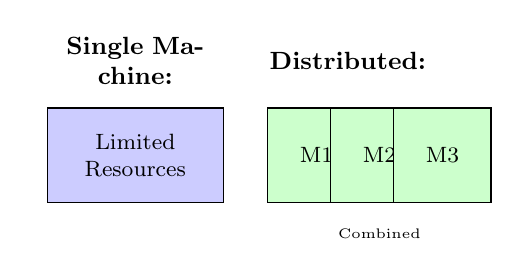
\begin{tikzpicture}[node distance=1.2cm, auto, scale=0.85, every node/.style={font=\footnotesize}]
    % Single machine
    \node[text width=2.5cm, align=center, font=\small] (single-label) {\textbf{Single Machine:}};
    \node[draw, rectangle, fill=blue!20, below of=single-label, text width=2cm, align=center, minimum height=1.2cm] (single) {Limited\\Resources};
    
    % Distributed
    \node[text width=2.5cm, align=center, font=\small, right of=single-label, xshift=1.5cm] (dist-label) {\textbf{Distributed:}};
    \node[draw, rectangle, fill=green!20, below of=dist-label, xshift=-0.4cm, text width=1cm, align=center, minimum height=1.2cm] (m1) {M1};
    \node[draw, rectangle, fill=green!20, below of=dist-label, xshift=0.4cm, text width=1cm, align=center, minimum height=1.2cm] (m2) {M2};
    \node[draw, rectangle, fill=green!20, below of=dist-label, xshift=1.2cm, text width=1cm, align=center, minimum height=1.2cm] (m3) {M3};
    \node[below of=m2, yshift=0.2cm, font=\tiny] {Combined};
\end{tikzpicture}
\end{center}
\end{frame}

\begin{frame}[fragile]{Client-Worker Architecture}
\textbf{Three Components:}

\begin{enumerate}
    \item \textbf{Client}: 
    \begin{itemize}
        \item Submits tasks
        \item Your Python session
        \item Coordinates computation
    \end{itemize}
    
    \item \textbf{Workers}: 
    \begin{itemize}
        \item Execute tasks
        \item Hold data in memory
        \item Report status to scheduler
    \end{itemize}
    
    \item \textbf{Scheduler}: 
    \begin{itemize}
        \item Coordinates execution
        \item Assigns tasks to workers
        \item Manages dependencies
    \end{itemize}
\end{enumerate}

\vspace{0.2cm}
\begin{center}
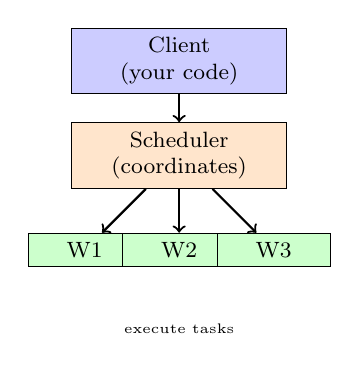
\begin{tikzpicture}[node distance=1.2cm, auto, scale=0.85, every node/.style={font=\footnotesize}]
    % Client
    \node[draw, rectangle, fill=blue!20, text width=2.5cm, align=center] (client) {Client\\(your code)};
    
    % Scheduler
    \node[draw, rectangle, fill=orange!20, below of=client, text width=2.5cm, align=center] (scheduler) {Scheduler\\(coordinates)};
    
    % Workers
    \node[draw, rectangle, fill=green!20, below of=scheduler, xshift=-1.2cm, text width=1.2cm, align=center] (w1) {W1};
    \node[draw, rectangle, fill=green!20, below of=scheduler, text width=1.2cm, align=center] (w2) {W2};
    \node[draw, rectangle, fill=green!20, below of=scheduler, xshift=1.2cm, text width=1.2cm, align=center] (w3) {W3};
    \node[below of=w2, yshift=0.2cm, font=\tiny] {execute tasks};
    
    % Edges
    \draw[->, thick] (client) -- (scheduler);
    \draw[->, thick] (scheduler) -- (w1);
    \draw[->, thick] (scheduler) -- (w2);
    \draw[->, thick] (scheduler) -- (w3);
\end{tikzpicture}
\end{center}
\end{frame}

\begin{frame}[fragile]{Creating a Client}
\begin{lstlisting}
from dask.distributed import Client

# Local cluster (single machine)
client = Client(n_workers=4)

# Remote cluster (multiple machines)
client = Client('tcp://scheduler-address:8786')
\end{lstlisting}

\textbf{Local vs Remote:}
\begin{itemize}
    \item \textbf{Local}: All on one machine (good for testing)
    \item \textbf{Remote}: Across multiple machines (production)
\end{itemize}

\vspace{0.3cm}
\textbf{Common Setup:}
\begin{itemize}
    \item Development: Local client
    \item Production: Remote cluster (EC2 instances)
\end{itemize}
\end{frame}

\begin{frame}[fragile]{Client Configuration}
\begin{lstlisting}
client = Client(
    n_workers=4,              # Number of worker processes
    threads_per_worker=2,     # Threads per worker
    memory_limit='8GB'        # Memory per worker
)
\end{lstlisting}

\textbf{Configuration Options:}
\begin{itemize}
    \item \texttt{n\_workers}: Number of worker processes
    \item \texttt{threads\_per\_worker}: Threads per worker
    \item \texttt{memory\_limit}: Memory limit per worker
    \item \texttt{processes}: Use processes vs threads
\end{itemize}

\vspace{0.3cm}
\textbf{Resource Planning:}
\begin{itemize}
    \item Balance workers vs threads
    \item Consider available memory
    \item Match to your workload
\end{itemize}
\end{frame}

\begin{frame}[fragile]{Workers and Cores}
\textbf{Worker Structure:}
\begin{itemize}
    \item Each worker = separate process
    \item Workers have cores (threads)
    \item Balance workers vs cores per worker
\end{itemize}

\vspace{0.3cm}
\textbf{Example:}
\begin{itemize}
    \item 8 CPU cores available
    \item Option 1: 4 workers $\times$ 2 threads = 8 threads
    \item Option 2: 8 workers $\times$ 1 thread = 8 threads
\end{itemize}

\vspace{0.3cm}
\begin{center}
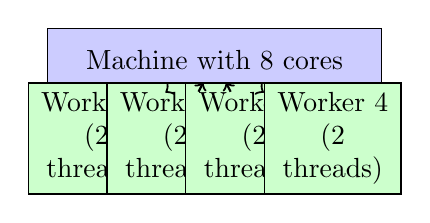
\begin{tikzpicture}[node distance=1cm, auto]
    % Machine
    \node[draw, rectangle, fill=blue!20, text width=4cm, align=center, minimum height=0.8cm] (machine) {Machine with 8 cores};
    
    % Workers
    \node[draw, rectangle, fill=green!20, below of=machine, xshift=-1.5cm, text width=1.5cm, align=center] (w1) {Worker 1\\(2 threads)};
    \node[draw, rectangle, fill=green!20, below of=machine, xshift=-0.5cm, text width=1.5cm, align=center] (w2) {Worker 2\\(2 threads)};
    \node[draw, rectangle, fill=green!20, below of=machine, xshift=0.5cm, text width=1.5cm, align=center] (w3) {Worker 3\\(2 threads)};
    \node[draw, rectangle, fill=green!20, below of=machine, xshift=1.5cm, text width=1.5cm, align=center] (w4) {Worker 4\\(2 threads)};
    
    % Edges
    \draw[->, thick] (machine) -- (w1);
    \draw[->, thick] (machine) -- (w2);
    \draw[->, thick] (machine) -- (w3);
    \draw[->, thick] (machine) -- (w4);
\end{tikzpicture}
\end{center}
\end{frame}

\begin{frame}{The Dashboard}
\textbf{Real-Time Monitoring:}
\begin{itemize}
    \item Task stream visualization
    \item Worker status
    \item Memory usage
    \item Performance metrics
\end{itemize}

\vspace{0.3cm}
\textbf{Access:}
\begin{itemize}
    \item URL shown when creating Client
    \item Usually: \texttt{http://localhost:8787/status}
    \item Opens in browser
\end{itemize}

\vspace{0.3cm}
\textbf{Key Views:}
\begin{itemize}
    \item Task Stream: See tasks executing
    \item Worker Memory: Memory usage per worker
    \item Progress: Overall computation progress
\end{itemize}
\end{frame}

\begin{frame}{Dashboard: Task Stream}
\textbf{What You See:}
\begin{itemize}
    \item Tasks executing over time
    \item Worker utilization
    \item Bottlenecks and idle time
    \item Task dependencies
\end{itemize}

\vspace{0.3cm}
\textbf{Use Cases:}
\begin{itemize}
    \item Identify performance bottlenecks
    \item See if workers are busy
    \item Understand computation flow
    \item Debug slow operations
\end{itemize}

\vspace{0.2cm}
\begin{center}
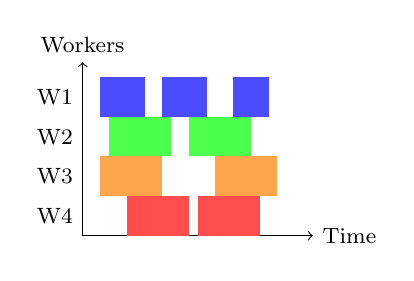
\begin{tikzpicture}[x=0.25cm, y=0.7cm, scale=0.9]
    % Timeline axis
    \draw[->] (0,0) -- (13,0) node[right, font=\footnotesize] {Time};
    \draw[->] (0,0) -- (0,3.5) node[above, font=\footnotesize] {Workers};
    
    % Worker labels
    \node[left, font=\footnotesize] at (0,2.8) {W1};
    \node[left, font=\footnotesize] at (0,2) {W2};
    \node[left, font=\footnotesize] at (0,1.2) {W3};
    \node[left, font=\footnotesize] at (0,0.4) {W4};
    
    % Tasks (color-coded by worker)
    \fill[blue!70] (1,2.4) rectangle (3.5,3.2);
    \fill[blue!70] (4.5,2.4) rectangle (7,3.2);
    \fill[blue!70] (8.5,2.4) rectangle (10.5,3.2);
    
    \fill[green!70] (1.5,1.6) rectangle (5,2.4);
    \fill[green!70] (6,1.6) rectangle (9.5,2.4);
    
    \fill[orange!70] (1,0.8) rectangle (4.5,1.6);
    \fill[orange!70] (7.5,0.8) rectangle (11,1.6);
    
    \fill[red!70] (2.5,0) rectangle (6,0.8);
    \fill[red!70] (6.5,0) rectangle (10,0.8);
\end{tikzpicture}
\end{center}
\end{frame}

\begin{frame}{Dashboard: Worker Memory}
\textbf{Memory Monitoring:}
\begin{itemize}
    \item Memory usage per worker
    \item Identify memory pressure
    \item Optimize partition sizes
    \item Prevent out-of-memory errors
\end{itemize}

\vspace{0.3cm}
\textbf{What to Look For:}
\begin{itemize}
    \item Workers near memory limit
    \item Uneven memory distribution
    \item Memory leaks
\end{itemize}

\vspace{0.2cm}
\begin{center}
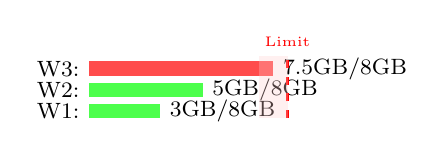
\begin{tikzpicture}[x=0.4cm, y=0.25cm, scale=0.9]
    % Worker 1
    \fill[green!70] (0,0) rectangle (2.5,0.8);
    \node[left, font=\footnotesize] at (0,0.4) {W1:};
    \node[right, font=\footnotesize] at (2.5,0.4) {3GB/8GB};
    
    % Worker 2
    \fill[green!70] (0,1.2) rectangle (4,2);
    \node[left, font=\footnotesize] at (0,1.6) {W2:};
    \node[right, font=\footnotesize] at (4,1.6) {5GB/8GB};
    
    % Worker 3
    \fill[red!70] (0,2.4) rectangle (6.5,3.2);
    \node[left, font=\footnotesize] at (0,2.8) {W3:};
    \node[right, font=\footnotesize] at (6.5,2.8) {7.5GB/8GB};
    
    % Limit line
    \draw[thick, red, dashed] (7,0) -- (7,3.5);
    \node[above, red, font=\tiny] at (7,3.5) {Limit};
    
    % Red zone indicator
    \fill[red!20, opacity=0.3] (6,0) rectangle (7,3.5);
\end{tikzpicture}
\end{center}
\end{frame}

\begin{frame}[fragile]{Performance Monitoring}
\begin{lstlisting}
# Get performance info
client.profile()      # Detailed profiling
client.nthreads()     # Total threads
client.ncores()       # Total cores
client.scheduler_info # Scheduler details
\end{lstlisting}

\textbf{Monitoring Tools:}
\begin{itemize}
    \item Client methods for info
    \item Dashboard for visualization
    \item Logs for debugging
\end{itemize}

\vspace{0.3cm}
\textbf{Key Metrics:}
\begin{itemize}
    \item Worker count
    \item Memory usage
    \item Task completion rate
    \item Network traffic
\end{itemize}
\end{frame}

\begin{frame}[fragile]{Persist vs Compute}
\begin{lstlisting}
# Compute: execute and return result
result = df.sum().compute()
# Result is a pandas Series (small)
# DataFrame is discarded

# Persist: execute and keep in memory
df_persisted = df.persist()
# DataFrame stays in memory
# Can reuse without recomputation
\end{lstlisting}

\textbf{When to Use:}
\begin{itemize}
    \item \textbf{Compute}: One-time results, final output
    \item \textbf{Persist}: Intermediate results, reused data
\end{itemize}

\vspace{0.2cm}
\begin{center}
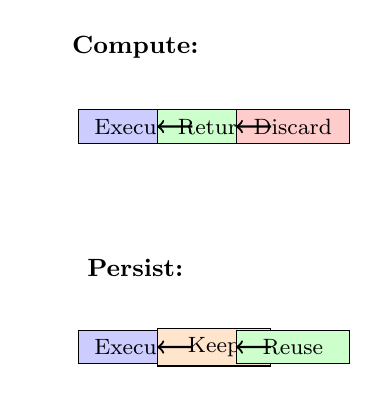
\begin{tikzpicture}[node distance=1cm, auto, scale=0.85, every node/.style={font=\footnotesize}]
    % Compute path
    \node[text width=2.5cm, align=center, font=\small] (comp-label) {\textbf{Compute:}};
    \node[draw, rectangle, fill=blue!20, below of=comp-label, text width=1.2cm, align=center] (exec1) {Execute};
    \node[draw, rectangle, fill=green!20, right of=exec1, text width=1.2cm, align=center] (ret1) {Return};
    \node[draw, rectangle, fill=red!20, right of=ret1, text width=1.2cm, align=center] (disc1) {Discard};
    \draw[->, thick] (exec1) -- (ret1);
    \draw[->, thick] (ret1) -- (disc1);
    
    % Persist path
    \node[text width=2.5cm, align=center, font=\small, below of=exec1, yshift=-0.8cm] (pers-label) {\textbf{Persist:}};
    \node[draw, rectangle, fill=blue!20, below of=pers-label, text width=1.2cm, align=center] (exec2) {Execute};
    \node[draw, rectangle, fill=orange!20, right of=exec2, text width=1.2cm, align=center] (keep) {Keep};
    \node[draw, rectangle, fill=green!20, right of=keep, text width=1.2cm, align=center] (reuse) {Reuse};
    \draw[->, thick] (exec2) -- (keep);
    \draw[->, thick] (keep) -- (reuse);
\end{tikzpicture}
\end{center}
\end{frame}

\begin{frame}[fragile]{Memory Management}
\textbf{Key Principles:}
\begin{itemize}
    \item Each worker has memory limit
    \item Partitions should fit in worker memory
    \item Monitor memory usage
    \item Use persist strategically
\end{itemize}

\vspace{0.3cm}
\textbf{Best Practices:}
\begin{itemize}
    \item Right-size partitions (100MB-1GB)
    \item Monitor dashboard
    \item Use persist for repeated computations
    \item Clear persisted data when done
\end{itemize}

\vspace{0.2cm}
\begin{center}
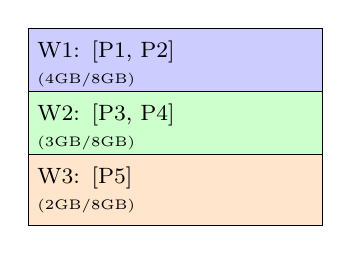
\begin{tikzpicture}[node distance=0.8cm, auto, scale=0.9, every node/.style={font=\footnotesize}]
    % Worker 1
    \node[draw, rectangle, fill=blue!20, text width=3.5cm, align=left, minimum height=0.9cm] (w1) {W1: [P1, P2]\\\tiny(4GB/8GB)};
    
    % Worker 2
    \node[draw, rectangle, fill=green!20, below of=w1, text width=3.5cm, align=left, minimum height=0.9cm] (w2) {W2: [P3, P4]\\\tiny(3GB/8GB)};
    
    % Worker 3
    \node[draw, rectangle, fill=orange!20, below of=w2, text width=3.5cm, align=left, minimum height=0.9cm] (w3) {W3: [P5]\\\tiny(2GB/8GB)};
\end{tikzpicture}
\end{center}
\end{frame}

\begin{frame}{Performance Optimization: Partitioning}
\textbf{Partitioning Strategy:}
\begin{itemize}
    \item Right-size partitions
    \item Align with worker memory
    \item Consider data locality
    \item Balance partition count
\end{itemize}

\vspace{0.3cm}
\textbf{Guidelines:}
\begin{itemize}
    \item 100MB-1GB per partition
    \item Match to worker memory
    \item More partitions = more parallelism (but more overhead)
    \item Fewer partitions = less overhead (but less parallelism)
\end{itemize}

\vspace{0.3cm}
\textbf{Example:}
\begin{itemize}
    \item 10GB dataset, 4 workers with 4GB each
    \item Good: 10-20 partitions of 500MB-1GB each
    \item Bad: 1000 partitions of 10MB each (too much overhead)
\end{itemize}
\end{frame}

\begin{frame}[fragile]{Performance Optimization: Caching}
\begin{lstlisting}
# Cache intermediate results
df_filtered = df[df['value'] > 100].persist()

# Reuse cached data
result1 = df_filtered.groupby('cat').sum()
result2 = df_filtered.groupby('cat').mean()
result3 = df_filtered.groupby('cat').count()
\end{lstlisting}

\textbf{Benefits:}
\begin{itemize}
    \item Avoid recomputation
    \item Faster subsequent operations
    \item Uses more memory
\end{itemize}

\vspace{0.2cm}
\begin{center}
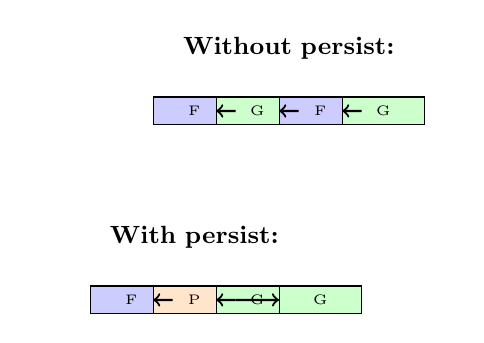
\begin{tikzpicture}[node distance=0.8cm, auto, scale=0.85, every node/.style={font=\footnotesize}]
    % Without persist
    \node[text width=4cm, align=center, font=\small] (no-label) {\textbf{Without persist:}};
    \node[draw, rectangle, fill=blue!20, below of=no-label, xshift=-1.2cm, text width=0.8cm, align=center, font=\tiny] (f1) {F};
    \node[draw, rectangle, fill=green!20, right of=f1, text width=0.8cm, align=center, font=\tiny] (g1) {G};
    \node[draw, rectangle, fill=blue!20, right of=g1, text width=0.8cm, align=center, font=\tiny] (f2) {F};
    \node[draw, rectangle, fill=green!20, right of=f2, text width=0.8cm, align=center, font=\tiny] (g2) {G};
    \draw[->, thick] (f1) -- (g1);
    \draw[->, thick] (g1) -- (f2);
    \draw[->, thick] (f2) -- (g2);
    
    % With persist
    \node[text width=4cm, align=center, font=\small, below of=f1, yshift=-0.8cm] (yes-label) {\textbf{With persist:}};
    \node[draw, rectangle, fill=blue!20, below of=yes-label, xshift=-0.8cm, text width=0.8cm, align=center, font=\tiny] (f3) {F};
    \node[draw, rectangle, fill=orange!20, right of=f3, text width=0.8cm, align=center, font=\tiny] (pers) {P};
    \node[draw, rectangle, fill=green!20, right of=pers, text width=0.8cm, align=center, font=\tiny] (g3) {G};
    \node[draw, rectangle, fill=green!20, right of=g3, text width=0.8cm, align=center, font=\tiny] (g4) {G};
    \draw[->, thick] (f3) -- (pers);
    \draw[->, thick] (pers) -- (g3);
    \draw[->, thick] (pers) -- (g4);
\end{tikzpicture}
\end{center}
\end{frame}

\begin{frame}{Debugging: Task Failures}
\textbf{When Tasks Fail:}
\begin{enumerate}
    \item Check dashboard for errors
    \item Review task status
    \item Check worker logs
    \item Look for error messages
\end{enumerate}

\vspace{0.3cm}
\textbf{Common Issues:}
\begin{itemize}
    \item Out of memory errors
    \item Network connectivity
    \item Data format issues
    \item Worker crashes
\end{itemize}

\vspace{0.3cm}
\textbf{Debugging Steps:}
\begin{enumerate}
    \item Check dashboard error view
    \item Review task tracebacks
    \item Check worker logs
    \item Verify data format
    \item Test with smaller data
\end{enumerate}
\end{frame}

\begin{frame}{Debugging: Slow Performance}
\textbf{Identifying Bottlenecks:}
\begin{itemize}
    \item Check task stream for idle workers
    \item Verify data locality (minimize network transfer)
    \item Check network bandwidth
    \item Look for straggler tasks
\end{itemize}

\vspace{0.3cm}
\textbf{Common Causes:}
\begin{itemize}
    \item Data shuffling (network transfer)
    \item Uneven partition sizes
    \item Worker overload
    \item Network latency
\end{itemize}

\vspace{0.3cm}
\textbf{Optimization Strategies:}
\begin{itemize}
    \item Co-locate data and computation
    \item Balance partition sizes
    \item Increase workers if CPU-bound
    \item Increase memory if memory-bound
\end{itemize}
\end{frame}

\begin{frame}{Scaling Considerations}
\textbf{Scaling Strategies:}
\begin{itemize}
    \item Add more workers (horizontal scaling)
    \item Increase worker memory (vertical scaling)
    \item Optimize data partitioning
    \item Consider data locality
\end{itemize}

\vspace{0.3cm}
\textbf{Trade-offs:}
\begin{itemize}
    \item More workers = more parallelism but more overhead
    \item Larger workers = more memory but fewer workers
    \item Network transfer can be bottleneck
\end{itemize}

\vspace{0.2cm}
\begin{center}
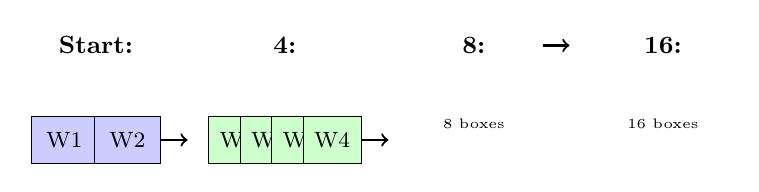
\begin{tikzpicture}[node distance=1.2cm, auto, scale=0.85, every node/.style={font=\footnotesize}]
    % Start
    \node[text width=1.5cm, align=center, font=\small] (start-label) {\textbf{Start:}};
    \node[draw, rectangle, fill=blue!20, below of=start-label, xshift=-0.4cm, text width=0.6cm, align=center, minimum height=0.6cm] (w1) {W1};
    \node[draw, rectangle, fill=blue!20, below of=start-label, xshift=0.4cm, text width=0.6cm, align=center, minimum height=0.6cm] (w2) {W2};
    
    % Arrow
    \draw[->, thick] (w2.east) -- ++(0.4,0);
    
    % Scale 1
    \node[text width=1.5cm, align=center, font=\small, right of=start-label, xshift=1.2cm] (scale1-label) {\textbf{4:}};
    \node[draw, rectangle, fill=green!20, below of=scale1-label, xshift=-0.6cm, text width=0.5cm, align=center, minimum height=0.6cm] (w3) {W1};
    \node[draw, rectangle, fill=green!20, below of=scale1-label, xshift=-0.2cm, text width=0.5cm, align=center, minimum height=0.6cm] (w4) {W2};
    \node[draw, rectangle, fill=green!20, below of=scale1-label, xshift=0.2cm, text width=0.5cm, align=center, minimum height=0.6cm] (w5) {W3};
    \node[draw, rectangle, fill=green!20, below of=scale1-label, xshift=0.6cm, text width=0.5cm, align=center, minimum height=0.6cm] (w6) {W4};
    
    % Arrow
    \draw[->, thick] (w6.east) -- ++(0.4,0);
    
    % Scale 2
    \node[text width=1.5cm, align=center, font=\small, right of=scale1-label, xshift=1.2cm] (scale2-label) {\textbf{8:}};
    \node[below of=scale2-label, yshift=0.2cm, font=\tiny] {8 boxes};
    
    % Arrow
    \draw[->, thick] (scale2-label.east) -- ++(0.4,0);
    
    % Scale 3
    \node[text width=1.5cm, align=center, font=\small, right of=scale2-label, xshift=1.2cm] (scale3-label) {\textbf{16:}};
    \node[below of=scale3-label, yshift=0.2cm, font=\tiny] {16 boxes};
\end{tikzpicture}
\end{center}
\end{frame}

\begin{frame}[fragile]{Connecting to EC2 Cluster}
\begin{lstlisting}
# On EC2 instance
from dask.distributed import Client

# Connect to scheduler
client = Client('tcp://scheduler-ip:8786')

# Or create local cluster on instance
client = Client(n_workers=4)
\end{lstlisting}

\textbf{EC2 Setup:}
\begin{itemize}
    \item Scheduler on one EC2 instance
    \item Workers on other EC2 instances
    \item Client can be anywhere (laptop, EC2, etc.)
\end{itemize}

\vspace{0.2cm}
\begin{center}
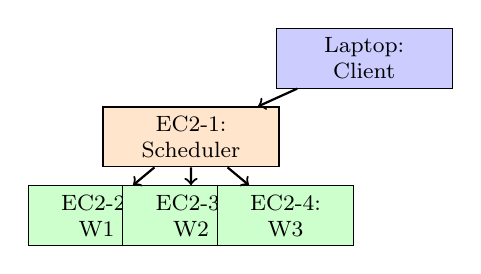
\begin{tikzpicture}[node distance=1cm, auto, scale=0.85, every node/.style={font=\footnotesize}]
    % Laptop
    \node[draw, rectangle, fill=blue!20, text width=2cm, align=center] (laptop) {Laptop:\\Client};
    
    % Scheduler
    \node[draw, rectangle, fill=orange!20, below of=laptop, xshift=-2.2cm, text width=2cm, align=center] (scheduler) {EC2-1:\\Scheduler};
    
    % Workers
    \node[draw, rectangle, fill=green!20, below of=scheduler, xshift=-1.2cm, text width=1.5cm, align=center] (w1) {EC2-2:\\W1};
    \node[draw, rectangle, fill=green!20, below of=scheduler, text width=1.5cm, align=center] (w2) {EC2-3:\\W2};
    \node[draw, rectangle, fill=green!20, below of=scheduler, xshift=1.2cm, text width=1.5cm, align=center] (w3) {EC2-4:\\W3};
    
    % Edges
    \draw[->, thick] (laptop) -- (scheduler);
    \draw[->, thick] (scheduler) -- (w1);
    \draw[->, thick] (scheduler) -- (w2);
    \draw[->, thick] (scheduler) -- (w3);
\end{tikzpicture}
\end{center}
\end{frame}

\begin{frame}{Best Practices}
\textbf{Resource Management:}
\begin{itemize}
    \item Right-size partitions
    \item Use persist strategically
    \item Monitor memory usage
    \item Clean up when done
\end{itemize}

\vspace{0.3cm}
\textbf{Performance:}
\begin{itemize}
    \item Monitor dashboard regularly
    \item Optimize data partitioning
    \item Minimize data shuffling
    \item Use appropriate number of workers
\end{itemize}

\vspace{0.3cm}
\textbf{Reliability:}
\begin{itemize}
    \item Handle errors gracefully
    \item Use try/except blocks
    \item Check task status
    \item Log important operations
\end{itemize}
\end{frame}

\begin{frame}{Summary}
\textbf{Key Takeaways:}
\begin{itemize}
    \item Distributed enables scaling beyond single machine
    \item Client coordinates workers via scheduler
    \item Dashboard provides real-time monitoring
    \item Optimize for your specific workload
\end{itemize}

\vspace{0.5cm}
\textbf{Next Steps:}
\begin{itemize}
    \item Practice with local cluster
    \item Explore dashboard features
    \item Optimize your workflows
    \item Scale to EC2 cluster
\end{itemize}

\vspace{0.3cm}
\textbf{Core Concepts:}
\begin{itemize}
    \item Client-Worker-Scheduler architecture
    \item Persist vs compute
    \item Memory management
    \item Performance optimization
\end{itemize}
\end{frame}

\end{document}

